\documentclass[letterpaper,10pt]{article}
\usepackage[margin=0.75in]{geometry}
\usepackage{amssymb}
\usepackage{amsmath}
\usepackage{setspace}
\usepackage{titlesec}
\usepackage{lipsum}
\usepackage{float}
\usepackage{physics}
\usepackage{subfig}
\usepackage{multicol}
\usepackage{graphicx}

\title{A Statistical Analysis of Cricket One Day Internationals}
\vspace{-0.35cm}
\author{\textbf{Author:}  Nikhil Lohia \\ 
\vspace{+0.15cm}
\\
  \textbf{Team Members:} \\
  Aishwarya Pratap Singh, Rahul Aakunuru \\
  and Ayushi Jain \\
  \vspace{-0.25cm}
  \small{Computer Science and Engineering Program} \\
  \vspace{-0.25cm}
  \footnotesize{School Of Computing, Informatics and Decision System Engineering}\\
  \vspace{-0.25cm}
  \footnotesize{Arizona State University, Tempe, AZ 85281}}

% \date{November 28, 2016}
\providecommand{\keywords}[1]{\textbf{\textit{Keywords---}} #1}
\begin{document}

\thispagestyle{empty}
\maketitle

\begin{multicols}{2}

\section{ABSTRACT}
\textit{Cricket is a game played in over a hundred countries worldwide; One Day International (ODI) is one of the most common forms played. Cricket enthusiasts may be interested in an easy-to-use method to see how their favorite team has been performing throughout the years, while sports analysts may be interested in seeing the trends of different teams' performances throughout the years. In our system, we propose a system of four simple visualizations that come together to tell a story of how the teams have been performing over the period of last 10 years and how their key players have contributed towards these results. The visualizations have been kept fairly simple and easy to understand keeping in mind the nature of audience the system targets.}\\ \\
\keywords{histogram, stacked area chart, cricket}

\section{INTRODUCTION}
Cricket is an extremely popular sport in the world today. The game attracts a huge audience and with it becoming extremely fast paced and increasingly competitive, performance analysis is steadily making its way into the teams dressing rooms. Data visualization and data analysis in cricket has increasingly become a critical part of the game. For instance, players can try to become technically better by analyzing their own performances. Second, teams can make plans for their upcoming matches by analyzing the performance of their competitors. Third, Selectors can analyze team performance to select appropriate teams. Finally, the International Cricket Council can analyze trends to maintain the level of the games taking place.\\
Each game of cricket can generate a lot of data that can be difficult to comprehend and analyze without some sort of visual representation. Thus, we have created a system of four interactive data visualizations in which users can explore team and player performance and discover under- lying trends in the data

\section{PROPOSED SOLUTION}
One of the main insights of our project is analyzing a player’s performance over the years. It was my responsibility to visualize this information and I used the concept of stacked area chart. Stacked area graphs are useful for comparing multiple variables changing over an interval and discover trends across a wide range of groups. I am using a spline-based area as it makes the graph look aesthetically pleasing. The years are presented on the X-Axis, whereas the Y-Axis shows the total number of runs scored.
\begin{figure}[H]
\begin{center}
{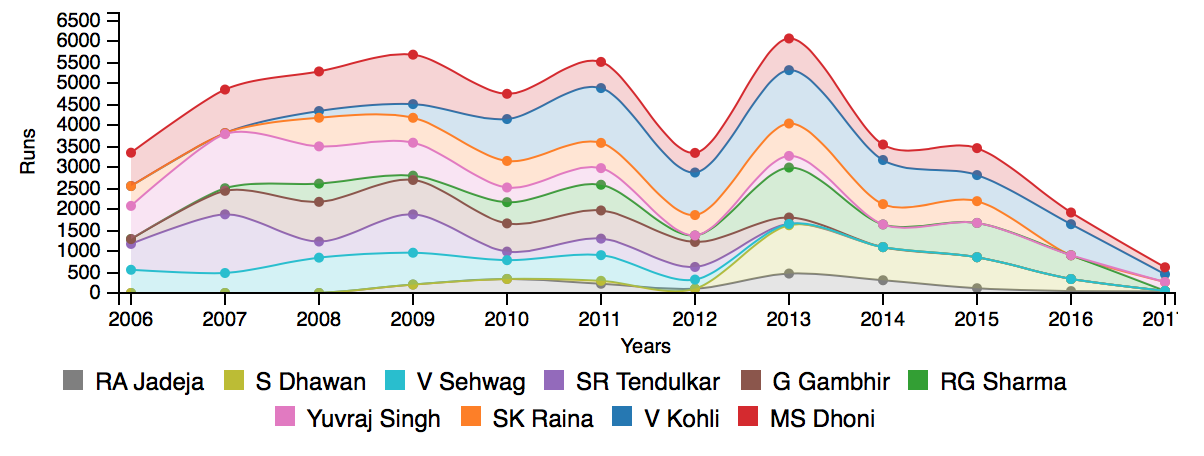
\includegraphics[width = 8cm]{stacked_area_chart.png}
\caption{Stacked Area Grapt for India}
}
\end{center}
\end{figure}
Stacked area chart is an extremely effective visualization in visualizing the performance of the team based on the sum of the number of runs, the players of the team, have been scoring each year. This also provides an effective means of analyzing the contribution made by a key batsman in the total number of runs scored. This visualization is useful in understanding when the team has peaked and coinciding this with the important tournaments played over the years gives us an understanding of the results of a lot them.\\
This visualization also helps analyze how the careers of individual players have evolved over the years. From the debuts and retirements of the players to injuries, that led to a temporary lapse in the performance of a player, can all be visualized using this visualization. \\
Each color in the graph represents a player and the width defines the number of runs scored by that specific player. The graph follows the Shneiderman's mantra as it gives an overview of the team's performance.

\section{RESULTS}
The stacked area chart in itself and along with the other visualizations can be used effectively to identify key insights related to the performance of a team and its players.
\begin{figure}[H]
\begin{center}
{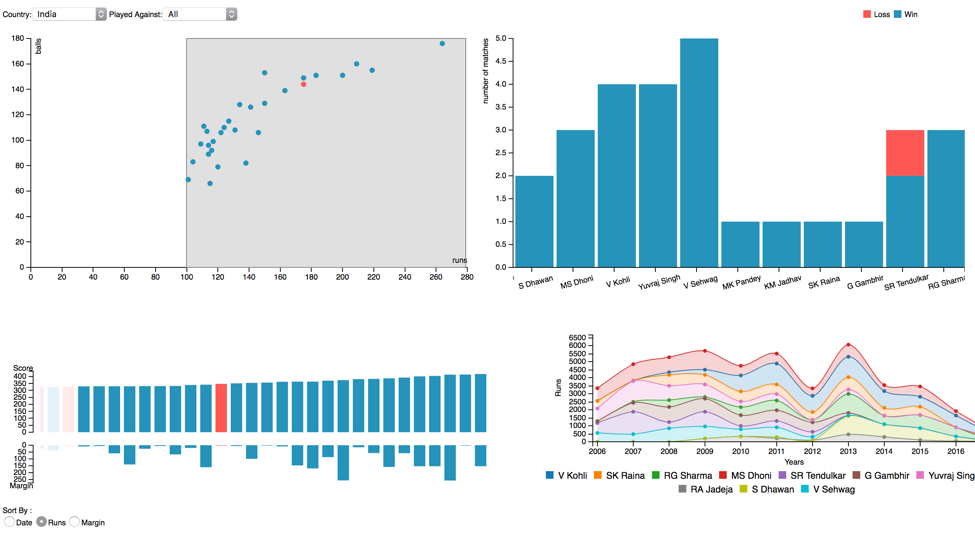
\includegraphics[width = 8cm]{case4.png}
\caption{System Overview}
}
\end{center}
\end{figure}

\subsection{What have been the causes for some of the excep- tionally good and exceptionally bad periods of performance of a team}
This case presents itself as a unique study of how the omission of some of the important players of the teams may explain why the team had a slump in their performance at a particular period. For instance, in the year $2016$, when three of the most prolific batsmen in the Sri Lankan cricket team, \textit{Jayawardene}, \textit{Sangakara} and \textit{Dilshan}, retired, their performance as team went down to an all time low in the last $10$ years.
\begin{figure}[H]
\begin{center}
{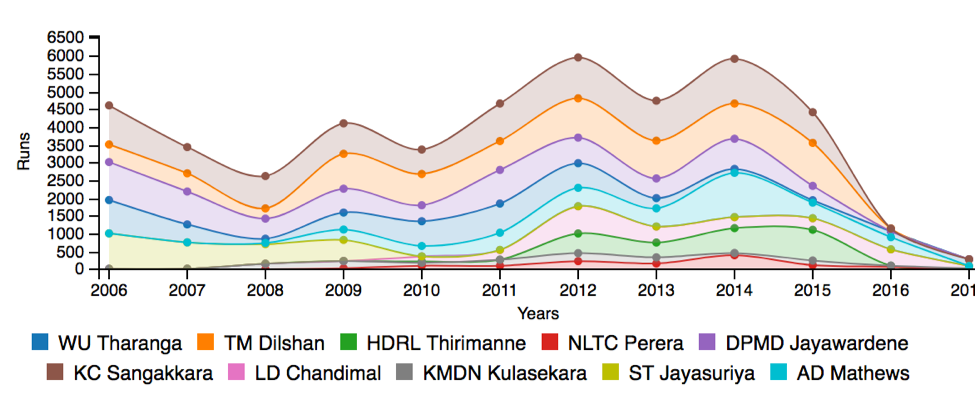
\includegraphics[width = 8cm]{sri_lanka_case.png}
\caption{Performance of Sri Lanka}
}
\end{center}
\end{figure}

\subsection{How were the champions made}
This case helps explain why certain teams have performed exceptionally well in some tournaments. India who were the winners of the International Cricket World Cup in the year $2011$ and the winners of the ICC Champions trophy in $2013$ were at the top of their performance in both those years. They however could not defend their title of the world champions in $2015$ due to an indifferent performance by the team. On the other hand, \textit{New Zealand} had an exceptionally good year as a team in $2015$ which resulted in them being one of the finalists in the World Cup. This was the first time ever that New Zealand had reached the finals in the tournament.

\begin{figure}[H]
\begin{center}
{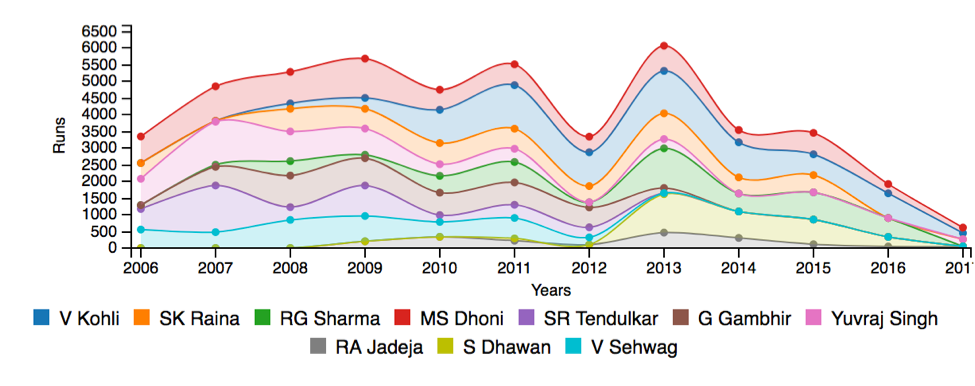
\includegraphics[width = 8cm]{india_case3.png}
\caption{Performance of India}
}
\end{center}
\end{figure}

\begin{figure}[H]
\begin{center}
{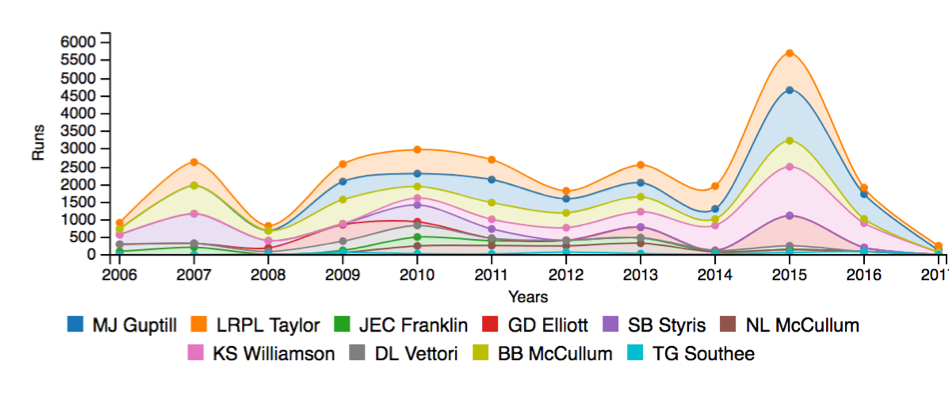
\includegraphics[width = 8cm]{newzealand_case3.png}
\caption{Performance of New Zealand}
}
\end{center}
\end{figure}

\section{KEY LEARNINGS}
A key learning from this project was that the amount of information that can be represented on a unit area of screen is very limited and with increasing it data becomes harder to fetch relevant insights from it. It is really important to express the information in such a way that the used does not get confused and is rather encouraged to explore insights on his own. We tried to explore how the strike rate defines a game outcome.\\
There are a few more metrics that go on to decide the outcome of a game, but it is interesting to see how with just the batting metric we can explain so many trends and results with respect to the teams. It can be an interesting endeavor to correlate our findings with some of the other metrics in the game.\\
We have also been able to explore D3, C3 and other related technologies while developing a fully functional system.


%\end{multicols}
%
%This is not multicol
%
%\begin{multicols}{2}

\section{CONCLUSION}
A good visualization is one which has interactivity and makes the comparison engaging. We present the viewer with data controls and let them uncover things on their own. We have presented a system that analyzes a team’s match plan by following Ben Shneiderman's information-seeking mantra\cite{mantra}. We focused on the fixed parameter of strike rate of a player. However, there still exists a challenge to extract information and gain insights from the bowling statistics of a team. Some teams are known for their exceptional spinners while others are known for players who can conceive all the wickets in a game. \\
Interactivity among the visualizations is a crucial part of our prototype. However, we may need to search for  similar  player  behavior  on  more abstract levels. We may want to know how players adapt their behavior when playing with others on their teams; player partnership may be a very interesting area of analysis. This could be another level of exploration.

\begin{thebibliography}{9}
\footnotesize
\setlength{\itemsep}{0pt}
\bibitem{latexcompanion}
M.~Goossens, F.~Mittelbach, A.~Samarin. \emph{The \LaTeX\ Companion},
Addison-Wesley (1994), ISBN~0-201-54199-8.

\bibitem{mantra}
Shneiderman, Ben. \emph{The eyes have it: A task by data type taxonomy for information visualizations.}, Visual Languages, 1996. Proceedings., IEEE Symposium on. IEEE, 1996.

\end{thebibliography}



\end{multicols}
\end{document}